\documentclass[answers]{exam}
\usepackage{../../mypackages}
\usepackage{../../macros}

%\usepackage{blindtext}

\SolutionEmphasis{\color{blue}}
\renewcommand{\solutiontitle}{\noindent}

\renewcommand{\arraystretch}{1.5} % Augmente l'espacement vertical entre les lignes du tableau
\newcolumntype{C}{>{\centering\arraybackslash}m{2cm}}

\SetLabelAlign{myright}{\hss\llap{$#1$}}
\newlist{where}{description}{1}
\setlist[where]{labelwidth=2cm,labelsep=1em,
                        leftmargin=!,align=myright,font=\normalfont}

\setlength{\parindent}{0pt}

\title{Interrogation N° - Sujet}
\author{N. Bancel}
\date{9 Janvier 2024}

\begin{document}


\textbf{Collège Lycée Suger}
\hfill
\textbf{Mathématiques / Physique-Chimie} \\

\textbf{Année 2024-2025}
\hfill
\textbf{1ères STD2A - 3èmes CI} \par

{\let\newpage\relax\maketitle}
%\maketitle

  
  {\let\newpage\relax\maketitle}

  \begin{center}
  \textbf{\textcolor{red}{Durée : 30 minutes. La calculatrice n'est pas autorisée}} \\
  \textbf{\textcolor{red}{Une réponse donnée sans justification sera considérée comme fausse.}} \\
  Cette interrogation contient \numquestions\ questions, sur \numpages\ pages et est notée sur 20 points. 
  
  \end{center}

\section*{Exercice 1}

\begin{figure}[H]
  \centering
  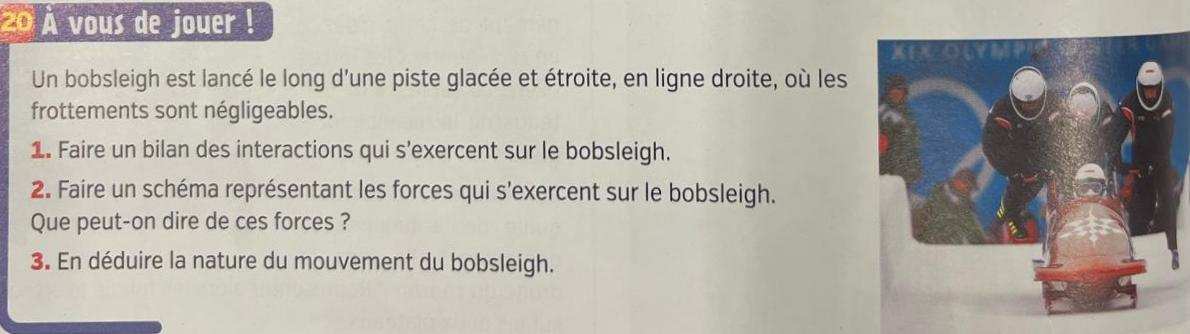
\includegraphics[width=0.5\linewidth]{img/test.jpg}
  \captionsetup{labelformat=empty}
  \caption{\label{} Bobsleigh}
\end{figure}

\begin{questions}

  \question[3] xxxx

  \begin{solution}
    yyyy
  \end{solution}

\question[3] xxxx

\begin{solution}
  yyyy
\end{solution}

\end{questions}


\section*{Exercice 2}
\end{document}
